\section{Eksperymenty}
W tym rozdziale opisane zostaną eksperymenty przeprowadzone w celu zbadania testów wydajnościowych środowisk uruchomieniowych. Testy zostały przeprowadzone na jednym komputerze wyposażonym w system operacyjny Linux, co pozwoliło na zminimalizowanie wpływu innych czynników na wyniki testów. 

\subsection{Algorytmy sortowania}
W celu zbadania wydajności danego środowiska uruchomieniowego, skonstruowana odpowiednie eksperymenty, które sprawdzają wydajność algorytmu sortowania. Wszystkie algorytmu sortowania zostały przetestowane dla każdego środowiska. W tabeli \ref{tab:sorting_experiments} przedstawiono ilość iteracji oraz ilość eksperymentów dla przeprowadzonych eksperymenty.

\begin{table}[H]
  \centering
  \begin{tabular}{|c|c|}
    \hline
    \textbf{Ilość iteracji} & \textbf{Ilość elementów} \\ \hline
    10 & 1000 \\ \hline
    100 & 1000 \\ \hline
    1000 & 1000 \\ \hline
    10 & 10000 \\ \hline
    100 & 10000 \\ \hline
    1000 & 10000 \\ \hline
  \end{tabular}
  \caption{Parametry eksperymentów}
  \label{tab:sorting_experiments}
\end{table}

\subsubsection{Wyniki - sortowanie bąbelkowe}
% 1
Na wykresie \ref{fig:bubble_sorting_e1} przedstawiono wyniki eksperymentu dla 10 iteracji oraz 1000 elementów dla algorytmów sortowania bąbelkowego napisanego w języku JavaScript. Na osi X przedstawia liczbę iteracji, na osi Y czas wykonania algorytmu w sekundach. 

\begin{figure}[H]
  \centering
  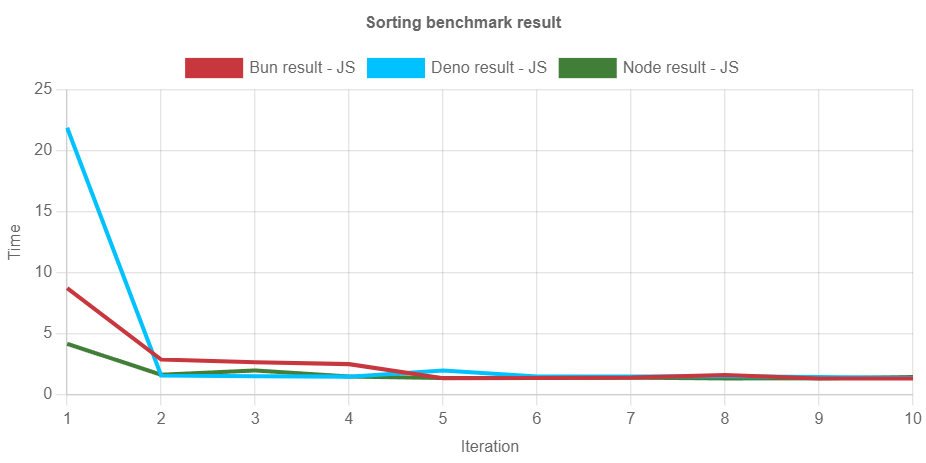
\includegraphics[width=0.7\textwidth]{Figures/sorting/bubble/e1_js.png}
  \caption{Wyniki eksperymentów dla algorytmu sortowania bąbelkowego dla 10 iteracji i 1000 elementów}
  \label{fig:bubble_sorting_e1}
\end{figure}

Na wykresie \ref{fig:bubble_sorting_e1_memory} przedstawiono wyniki eksperymentów dla algorytmu sortowania bąbelkowego dla 10 iteracji oraz 1000 elementów napisanego w języku JavaScript. Na osi X przedstawiono liczbę iteracji, natomiast na osi Y wykorzystanie pamięci w kilobytach. Jak widać, czas wykonania algorytmu rośnie wraz z ilością elementów.
\begin{figure}[H]
  \centering
  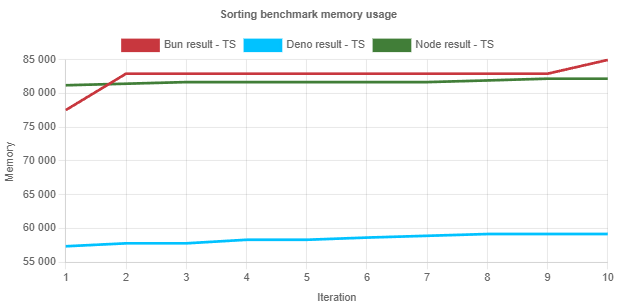
\includegraphics[width=0.7\textwidth]{Figures/sorting/bubble/e1_memory_ts.png}
  \caption{Wyniki eksperymentów dla algorytmu sortowania bąbelkowego dla 10 iteracji i 1000 elementów}
  \label{fig:bubble_sorting_e1_memory}
\end{figure}

Na wykresie \ref{fig:bubble_sorting_e1_ts} przedstawiono wyniki eksperymentu dla 10 iteracji oraz 1000 elementów dla algorytmów sortowania bąbelkowego napisanego w języku TypeScript. Na osi X przedstawia liczbę iteracji, na osi Y czas wykonania algorytmu w sekundach.

\begin{figure}[H]
  \centering
  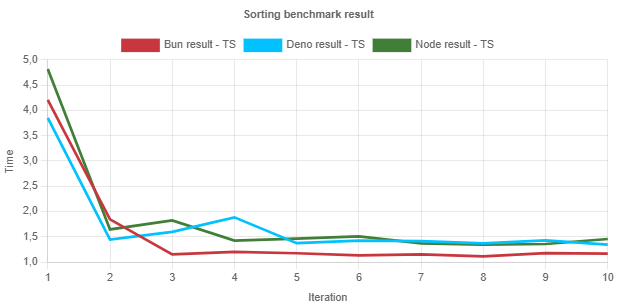
\includegraphics[width=0.8\textwidth]{Figures/sorting/bubble/e1_ts.png}
  \caption{Wyniki eksperymentów dla algorytmu sortowania bąbelkowego dla 10 iteracji i 1000 elementów}
  \label{fig:bubble_sorting_e1_ts}
\end{figure}

Na wykresie \ref{fig:bubble_sorting_e1_memory_ts} przedstawiono wyniki eksperymentów dla algorytmu sortowania bąbelkowego dla 10 iteracji i 1000 elementów napisanego w języku TypeScript. Na osi X przedstawiono liczbę iteracji, natomiast na osi Y wykorzystanie pamięci w kilobytach. Jak widać, czas wykonania algorytmu rośnie wraz z ilością elementów.
\begin{figure}[H]
  \centering
  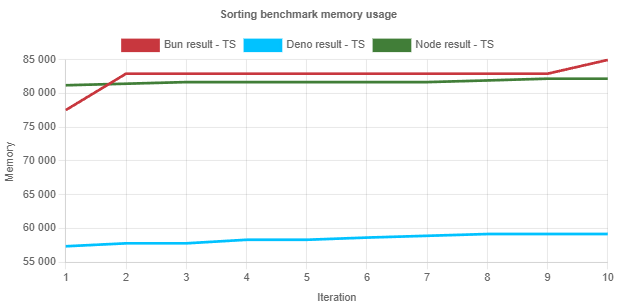
\includegraphics[width=0.8\textwidth]{Figures/sorting/bubble/e1_memory_ts.png}
  \caption{Wyniki eksperymentów dla algorytmu sortowania bąbelkowego dla 10 iteracji i 1000 elementów}
  \label{fig:bubble_sorting_e1_memory_ts}
\end{figure}

% 2
Na wykresie \ref{fig:bubble_sorting_e2} przedstawiono wyniki eksperymentu dla 10 iteracji oraz 1000 elementów dla algorytmów sortowania bąbelkowego napisanego w języku JavaScript. Na osi X przedstawia liczbę iteracji, na osi Y czas wykonania algorytmu w sekundach. 

\begin{figure}[H]
  \centering
  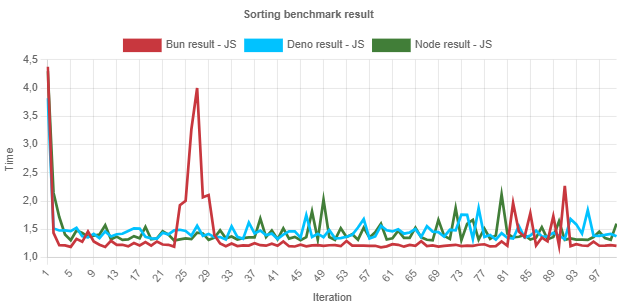
\includegraphics[width=0.8\textwidth]{Figures/sorting/bubble/e2_js.png}
  \caption{Wyniki eksperymentów dla algorytmu sortowania bąbelkowego dla 10 iteracji i 1000 elementów}
  \label{fig:bubble_sorting_e2}
\end{figure}

Na wykresie \ref{fig:bubble_sorting_e2_memory_js} przedstawiono wyniki eksperymentów dla algorytmu sortowania bąbelkowego dla 10 iteracji oraz 1000 elementów napisanego w języku JavaScript. Na osi X przedstawiono liczbę iteracji, natomiast na osi Y wykorzystanie pamięci w kilobytach. Jak widać, czas wykonania algorytmu rośnie wraz z ilością elementów.
\begin{figure}[H]
  \centering
  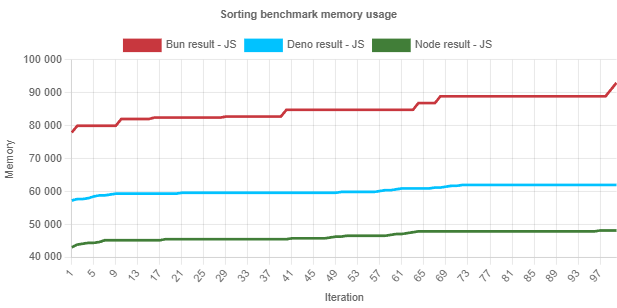
\includegraphics[width=0.8\textwidth]{Figures/sorting/bubble/e2_memory_js.png}
  \caption{Wyniki eksperymentów dla algorytmu sortowania bąbelkowego dla 100 iteracji i 1000 elementów}
  \label{fig:bubble_sorting_e2_memory_js}
\end{figure}

Na wykresie \ref{fig:bubble_sorting_e2_ts} przedstawiono wyniki eksperymentu dla 100 iteracji oraz 1000 elementów dla algorytmów sortowania bąbelkowego napisanego w języku TypeScript. Na osi X przedstawia liczbę iteracji, na osi Y czas wykonania algorytmu w sekundach. 

\begin{figure}[H]
  \centering
  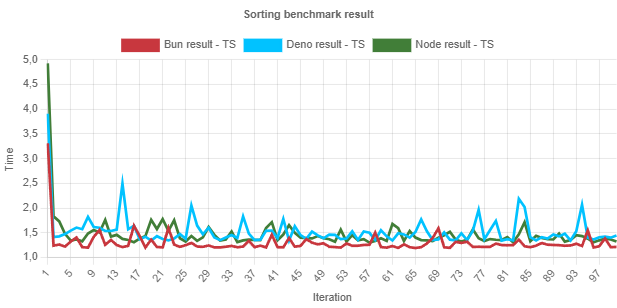
\includegraphics[width=0.8\textwidth]{Figures/sorting/bubble/e2_ts.png}
  \caption{Wyniki eksperymentów dla algorytmu sortowania bąbelkowego dla 100 iteracji i 1000 elementów}
  \label{fig:bubble_sorting_e2_ts}
\end{figure}

Na wykresie \ref{fig:bubble_sorting_e2_memory_ts} przedstawiono wyniki eksperymentów dla algorytmu sortowania bąbelkowego dla 100 iteracji i 1000 elementów napisanego w języku TypeScript. Na osi X przedstawiono liczbę iteracji, natomiast na osi Y wykorzystanie pamięci w kilobytach. Jak widać, czas wykonania algorytmu rośnie wraz z ilością elementów.
\begin{figure}[H]
  \centering
  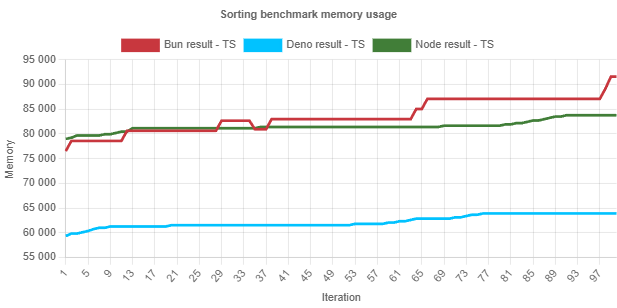
\includegraphics[width=0.8\textwidth]{Figures/sorting/bubble/e2_memory_ts.png}
  \caption{Wyniki eksperymentów dla algorytmu sortowania bąbelkowego dla 100 iteracji i 1000 elementów}
  \label{fig:bubble_sorting_e2_memory_ts}
\end{figure}

% 3
Na wykresie \ref{fig:bubble_sorting_e3} przedstawiono wyniki eksperymentów dla algorytmu sortowania bąbelkowego dla 1000 iteracji oraz 1000 elementów napisanego w języku JavaScript. Na osi X przedstawiono liczbę iteracji, natomiast na osi Y wykorzystanie pamięci w kilobytach. Jak widać, czas wykonania algorytmu rośnie wraz z ilością elementów.
\begin{figure}[H]
  \centering
  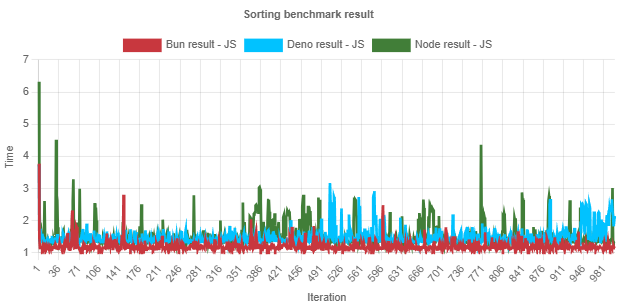
\includegraphics[width=0.8\textwidth]{Figures/sorting/bubble/e3_js.png}
  \caption{Wyniki eksperymentów dla algorytmu sortowania bąbelkowego dla 1000 iteracji i 1000 elementów}
  \label{fig:bubble_sorting_e3}
\end{figure}

Na wykresie \ref{fig:bubble_sorting_e3_memory_js} przedstawiono wyniki eksperymentów dla algorytmu sortowania bąbelkowego dla 1000 iteracji oraz 1000 elementów napisanego w języku JavaScript. Na osi X przedstawiono liczbę iteracji, natomiast na osi Y wykorzystanie pamięci w kilobytach. Jak widać, czas wykonania algorytmu rośnie wraz z ilością elementów.
\begin{figure}[H]
  \centering
  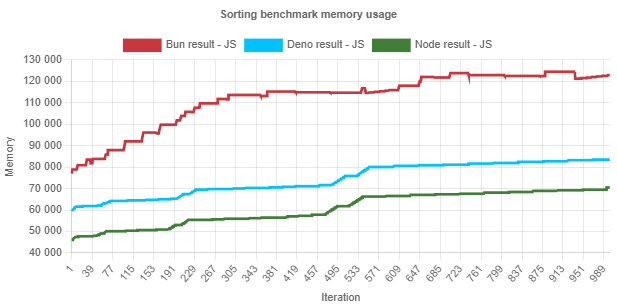
\includegraphics[width=0.8\textwidth]{Figures/sorting/bubble/e3_memory_js.png}
  \caption{Wyniki eksperymentów dla algorytmu sortowania bąbelkowego dla 1000 iteracji i 1000 elementów}
  \label{fig:bubble_sorting_e3_memory_js}
\end{figure}

Na wykresie \ref{fig:bubble_sorting_e3_ts} przedstawiono wyniki eksperymentu dla 1000 iteracji oraz 1000 elementów dla algorytmów sortowania bąbelkowego, napisanego w języku TypeScript. Na osi X przedstawia liczbę iteracji, na osi Y czas wykonania algorytmu w sekundach. 

\begin{figure}[H]
  \centering
  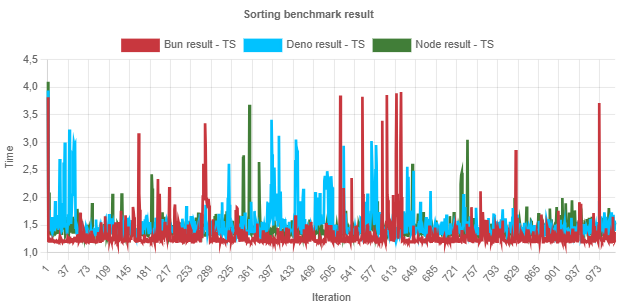
\includegraphics[width=0.8\textwidth]{Figures/sorting/bubble/e3_ts.png}
  \caption{Wyniki eksperymentów dla algorytmu sortowania bąbelkowego dla 1000 iteracji i 1000 elementów}
  \label{fig:bubble_sorting_e3_ts}
\end{figure}

Na wykresie \ref{fig:bubble_sorting_e3_memory_ts} przedstawiono wyniki eksperymentów dla algorytmu sortowania bąbelkowego. Na osi X przedstawiono liczbę iteracji, natomiast na osi Y wykorzystanie pamięci w kilobytach. Jak widać, czas wykonania algorytmu rośnie wraz z ilością elementów.
\begin{figure}[H]
  \centering
  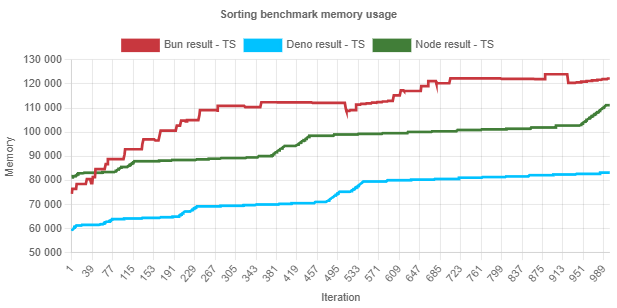
\includegraphics[width=0.8\textwidth]{Figures/sorting/bubble/e3_memory_ts.png}
  \caption{Wyniki eksperymentów dla algorytmu sortowania bąbelkowego dla 1000 iteracji i 1000 elementów}
  \label{fig:bubble_sorting_e3_memory_ts}
\end{figure}

%4
Na wykresie \ref{fig:bubble_sorting_e4} przedstawiono wyniki eksperymentów dla algorytmu sortowania bąbelkowego. Na osi X przedstawiono liczbę iteracji, natomiast na osi Y wykorzystanie pamięci w kilobytach. Jak widać, czas wykonania algorytmu rośnie wraz z ilością elementów.
\begin{figure}[H]
  \centering
  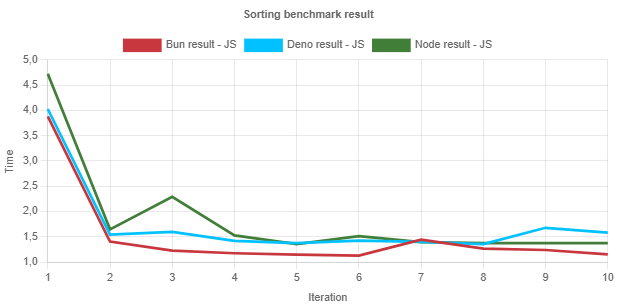
\includegraphics[width=0.8\textwidth]{Figures/sorting/bubble/e4_js.png}
  \caption{Wyniki eksperymentów dla algorytmu sortowania bąbelkowego dla 10 iteracji i 10000 elementów}
  \label{fig:bubble_sorting_e4}
\end{figure}

Na wykresie \ref{fig:bubble_sorting_e4_memory_js} przedstawiono wyniki eksperymentów dla algorytmu sortowania bąbelkowego. Na osi X przedstawiono liczbę iteracji, natomiast na osi Y wykorzystanie pamięci w kilobytach. Jak widać, czas wykonania algorytmu rośnie wraz z ilością elementów.
\begin{figure}[H]
  \centering
  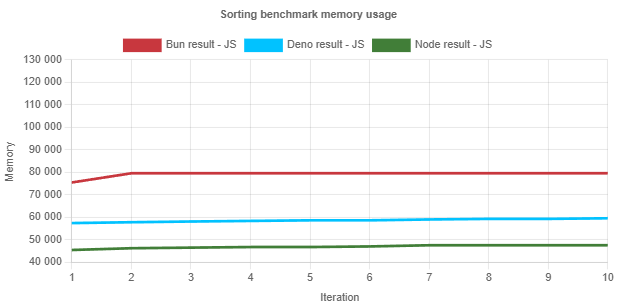
\includegraphics[width=0.8\textwidth]{Figures/sorting/bubble/e4_memory_js.png}
  \caption{Wyniki eksperymentów dla algorytmu sortowania bąbelkowego dla 10 iteracji i 10000 elementów}
  \label{fig:bubble_sorting_e4_memory_js}
\end{figure}

Na wykresie \ref{fig:bubble_sorting_e4_ts} przedstawiono wyniki eksperymentu dla 100 iteracji oraz 1000 elementów dla algorytmów sortowania bąbelkowego. Na osi X przedstawia liczbę iteracji, na osi Y czas wykonania algorytmu w sekundach. 

\begin{figure}[H]
  \centering
  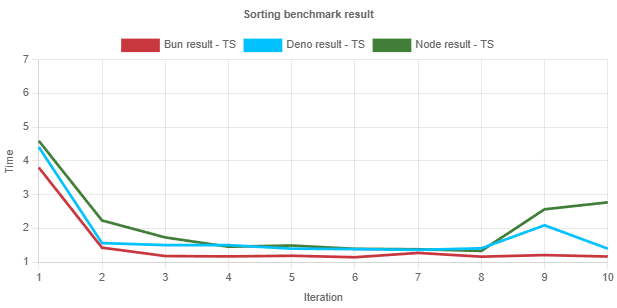
\includegraphics[width=0.8\textwidth]{Figures/sorting/bubble/e4_ts.png}
  \caption{Wyniki eksperymentów dla algorytmu sortowania bąbelkowego dla 10 iteracji i 10000 elementów}
  \label{fig:bubble_sorting_e4_ts}
\end{figure}

Na wykresie \ref{fig:bubble_sorting_e4_memory_ts} przedstawiono wyniki eksperymentów dla algorytmu sortowania bąbelkowego. Na osi X przedstawiono liczbę iteracji, natomiast na osi Y wykorzystanie pamięci w kilobytach. Jak widać, czas wykonania algorytmu rośnie wraz z ilością elementów.
\begin{figure}[H]
  \centering
  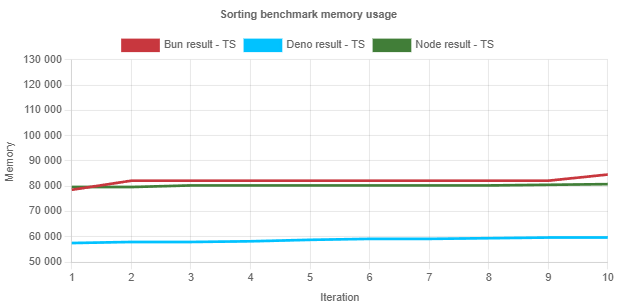
\includegraphics[width=0.8\textwidth]{Figures/sorting/bubble/e4_memory_ts.png}
  \caption{Wyniki eksperymentów dla algorytmu sortowania bąbelkowego dla 10 iteracji i 10000 elementów}
  \label{fig:bubble_sorting_e4_memory_ts}
\end{figure}

% 5
Na wykresie \ref{fig:bubble_sorting_e5} przedstawiono wyniki eksperymentów dla algorytmu sortowania bąbelkowego. Na osi X przedstawiono liczbę iteracji, natomiast na osi Y wykorzystanie pamięci w kilobytach. Jak widać, czas wykonania algorytmu rośnie wraz z ilością elementów.
\begin{figure}[H]
  \centering
  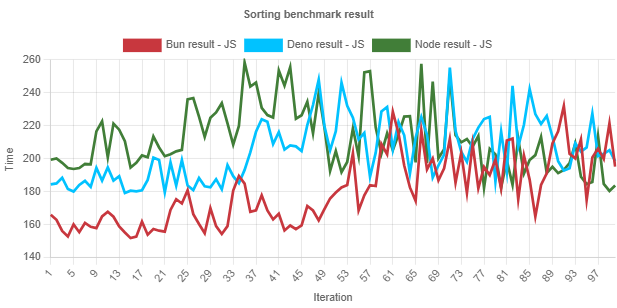
\includegraphics[width=0.8\textwidth]{Figures/sorting/bubble/e5_js.png}
  \caption{Wyniki eksperymentów dla algorytmu sortowania bąbelkowego dla 100 iteracji i 10000 elementów}
  \label{fig:bubble_sorting_e5}
\end{figure}

Na wykresie \ref{fig:bubble_sorting_e5_memory_js} przedstawiono wyniki eksperymentów dla algorytmu sortowania bąbelkowego. Na osi X przedstawiono liczbę iteracji, natomiast na osi Y wykorzystanie pamięci w kilobytach. Jak widać, czas wykonania algorytmu rośnie wraz z ilością elementów.
\begin{figure}[H]
  \centering
  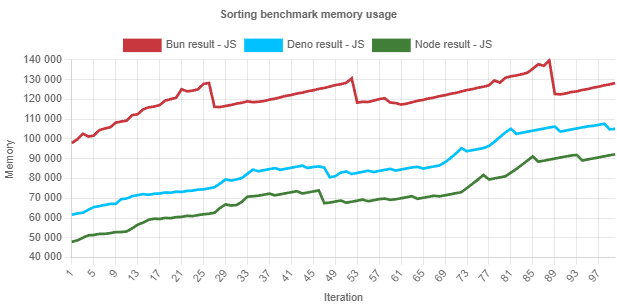
\includegraphics[width=0.8\textwidth]{Figures/sorting/bubble/e5_memory_js.png}
  \caption{Wyniki eksperymentów dla algorytmu sortowania bąbelkowego dla 100 iteracji i 10000 elementów}
  \label{fig:bubble_sorting_e5_memory_js}
\end{figure}

Na wykresie \ref{fig:bubble_sorting_e5_ts} przedstawiono wyniki eksperymentu dla 100 iteracji oraz 1000 elementów dla algorytmów sortowania bąbelkowego. Na osi X przedstawia liczbę iteracji, na osi Y czas wykonania algorytmu w sekundach. 

\begin{figure}[H]
  \centering
  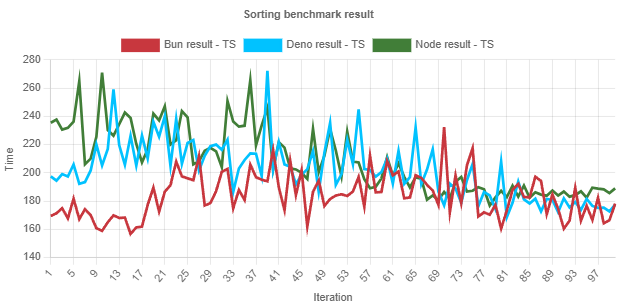
\includegraphics[width=0.8\textwidth]{Figures/sorting/bubble/e5_ts.png}
  \caption{Wyniki eksperymentów dla algorytmu sortowania bąbelkowego dla 100 iteracji i 10000 elementów}
  \label{fig:bubble_sorting_e5_ts}
\end{figure}

Na wykresie \ref{fig:bubble_sorting_e5_memory_ts} przedstawiono wyniki eksperymentów dla algorytmu sortowania bąbelkowego. Na osi X przedstawiono liczbę iteracji, natomiast na osi Y wykorzystanie pamięci w kilobytach. Jak widać, czas wykonania algorytmu rośnie wraz z ilością elementów.
\begin{figure}[H]
  \centering
  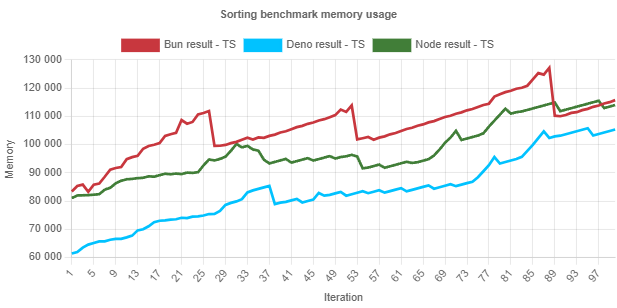
\includegraphics[width=0.8\textwidth]{Figures/sorting/bubble/e5_memory_ts.png}
  \caption{Wyniki eksperymentów dla algorytmu sortowania bąbelkowego dla 100 iteracji i 10000 elementów}
  \label{fig:bubble_sorting_e5_memory_ts}
\end{figure}

% 6
Na wykresie \ref{fig:bubble_sorting_e6} przedstawiono wyniki eksperymentów dla algorytmu sortowania bąbelkowego. Na osi X przedstawiono liczbę iteracji, natomiast na osi Y wykorzystanie pamięci w kilobytach. Jak widać, czas wykonania algorytmu rośnie wraz z ilością elementów.
\begin{figure}[H]
  \centering
  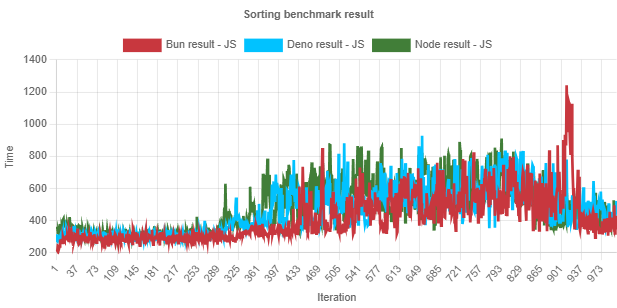
\includegraphics[width=0.8\textwidth]{Figures/sorting/bubble/e6_js.png}
  \caption{Wyniki eksperymentów dla algorytmu sortowania bąbelkowego dla 1000 iteracji i 10000 elementów}
  \label{fig:bubble_sorting_e6}
\end{figure}

Na wykresie \ref{fig:bubble_sorting_e6_memory_js} przedstawiono wyniki eksperymentów dla algorytmu sortowania bąbelkowego. Na osi X przedstawiono liczbę iteracji, natomiast na osi Y wykorzystanie pamięci w kilobytach. Jak widać, czas wykonania algorytmu rośnie wraz z ilością elementów.
\begin{figure}[H]
  \centering
  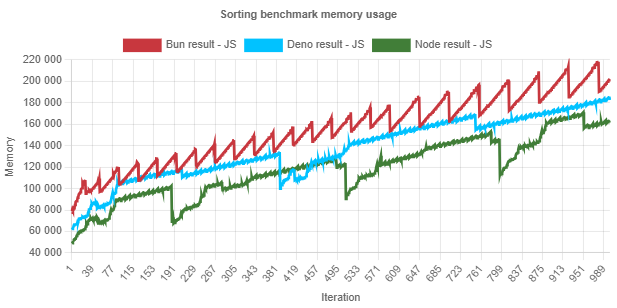
\includegraphics[width=0.8\textwidth]{Figures/sorting/bubble/e6_memory_js.png}
  \caption{Wyniki eksperymentów dla algorytmu sortowania bąbelkowego dla 1000 iteracji i 10000 elementów}
  \label{fig:bubble_sorting_e6_memory_js}
\end{figure}

Na wykresie \ref{fig:bubble_sorting_e6_ts} przedstawiono wyniki eksperymentu dla 100 iteracji oraz 1000 elementów dla algorytmów sortowania bąbelkowego. Na osi X przedstawia liczbę iteracji, na osi Y czas wykonania algorytmu w sekundach. 

\begin{figure}[H]
  \centering
  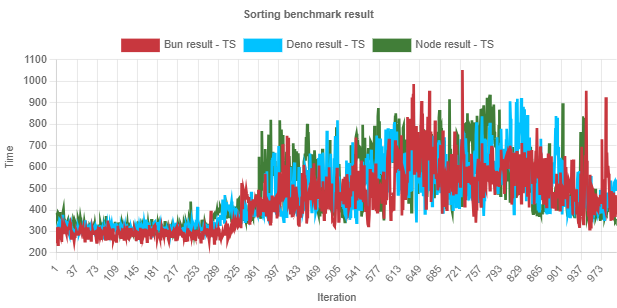
\includegraphics[width=0.8\textwidth]{Figures/sorting/bubble/e6_ts.png}
  \caption{Wyniki eksperymentów dla algorytmu sortowania bąbelkowego dla 1000 iteracji i 10000 elementów}
  \label{fig:bubble_sorting_e6_ts}
\end{figure}

Na wykresie \ref{fig:bubble_sorting_e6_memory_ts} przedstawiono wyniki eksperymentów dla algorytmu sortowania bąbelkowego. Na osi X przedstawiono liczbę iteracji, natomiast na osi Y wykorzystanie pamięci w kilobytach. Jak widać, czas wykonania algorytmu rośnie wraz z ilością elementów.
\begin{figure}[H]
  \centering
  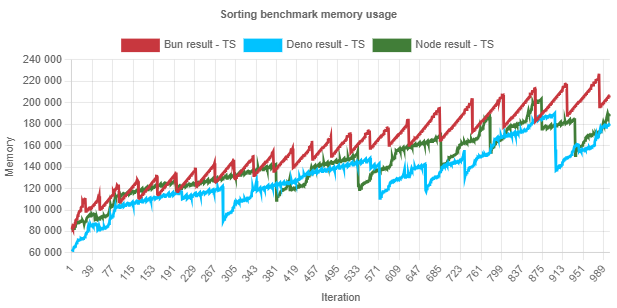
\includegraphics[width=0.8\textwidth]{Figures/sorting/bubble/e6_memory_ts.png}
  \caption{Wyniki eksperymentów dla algorytmu sortowania bąbelkowego dla 1000 iteracji i 10000 elementów}
  \label{fig:bubble_sorting_e6_memory_ts}
\end{figure}

\subsubsection{Wyniki - sortowanie szybkie}
Na wykresie \ref{fig:quick_sorting_e1_js} przedstawiono wyniki eksperymentu dla 10 iteracji oraz 1000 elementów dla algorytmów sortowania szybkiego napisanego w języku JavaScript. Na osi X przedstawia liczbę iteracji, na osi Y czas wykonania algorytmu w sekundach. 

\begin{figure}[H]
  \centering
  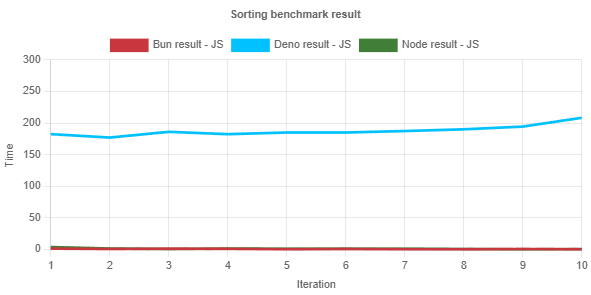
\includegraphics[width=0.7\textwidth]{Figures/sorting/quick/e1_js.png}
  \caption{Wyniki eksperymentów dla algorytmu sortowania szybkiego dla 10 iteracji i 1000 elementów}
  \label{fig:quick_sorting_e1_js}
\end{figure}

Na wykresie \ref{fig:quick_sorting_e1_memory_js} przedstawiono wyniki eksperymentów dla algorytmu sortowania bąbelkowego dla 10 iteracji oraz 1000 elementów napisanego w języku JavaScript. Na osi X przedstawiono liczbę iteracji, natomiast na osi Y wykorzystanie pamięci w kilobytach. Jak widać, czas wykonania algorytmu rośnie wraz z ilością elementów.
\begin{figure}[H]
  \centering
  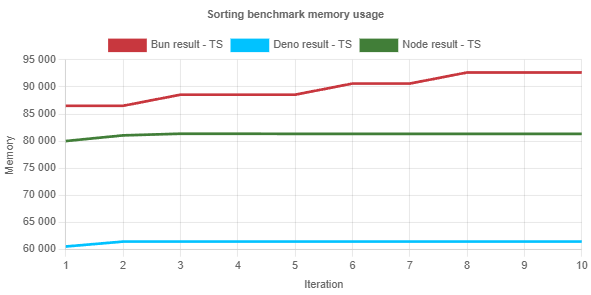
\includegraphics[width=0.7\textwidth]{Figures/sorting/quick/e1_memory_ts.png}
  \caption{Wyniki eksperymentów dla algorytmu sortowania bąbelkowego dla 10 iteracji i 1000 elementów}
  \label{fig:quick_sorting_e1_memory_js}
\end{figure}

Na wykresie \ref{fig:quick_sorting_e1_ts} przedstawiono wyniki eksperymentu dla 10 iteracji oraz 1000 elementów dla algorytmów sortowania bąbelkowego napisanego w języku TypeScript. Na osi X przedstawia liczbę iteracji, na osi Y czas wykonania algorytmu w sekundach.

\begin{figure}[H]
  \centering
  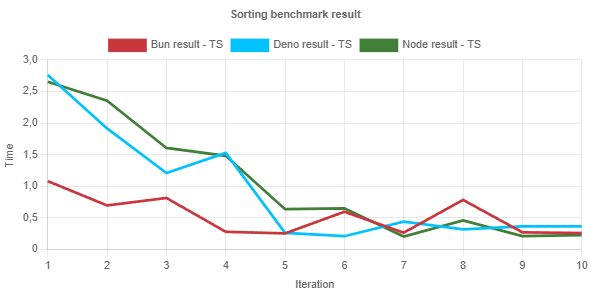
\includegraphics[width=0.8\textwidth]{Figures/sorting/quick/e1_ts.png}
  \caption{Wyniki eksperymentów dla algorytmu sortowania bąbelkowego dla 10 iteracji i 1000 elementów}
  \label{fig:quick_sorting_e1_ts}
\end{figure}

Na wykresie \ref{fig:quick_sorting_e1_memory_ts} przedstawiono wyniki eksperymentów dla algorytmu sortowania bąbelkowego dla 10 iteracji i 1000 elementów napisanego w języku TypeScript. Na osi X przedstawiono liczbę iteracji, natomiast na osi Y wykorzystanie pamięci w kilobytach. Jak widać, czas wykonania algorytmu rośnie wraz z ilością elementów.
\begin{figure}[H]
  \centering
  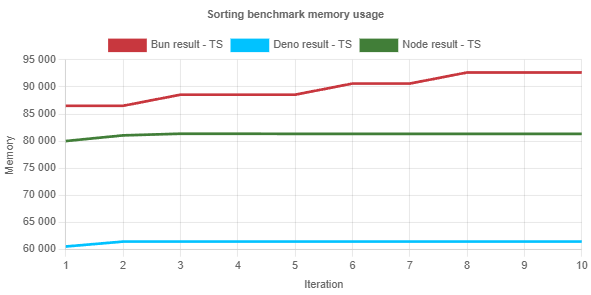
\includegraphics[width=0.8\textwidth]{Figures/sorting/quick/e1_memory_ts.png}
  \caption{Wyniki eksperymentów dla algorytmu sortowania bąbelkowego dla 10 iteracji i 1000 elementów}
  \label{fig:quick_sorting_e1_memory_ts}
\end{figure}

% 2
Na wykresie \ref{fig:quick_sorting_e2} przedstawiono wyniki eksperymentu dla 10 iteracji oraz 1000 elementów dla algorytmów sortowania bąbelkowego napisanego w języku JavaScript. Na osi X przedstawia liczbę iteracji, na osi Y czas wykonania algorytmu w sekundach. 

\begin{figure}[H]
  \centering
  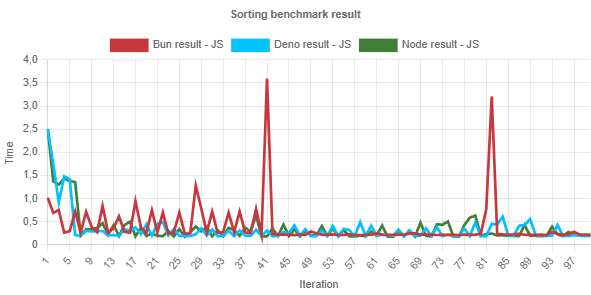
\includegraphics[width=0.8\textwidth]{Figures/sorting/quick/e2_js.png}
  \caption{Wyniki eksperymentów dla algorytmu sortowania bąbelkowego dla 10 iteracji i 1000 elementów}
  \label{fig:quick_sorting_e2}
\end{figure}

Na wykresie \ref{fig:quick_sorting_e2_memory_js} przedstawiono wyniki eksperymentów dla algorytmu sortowania bąbelkowego dla 10 iteracji oraz 1000 elementów napisanego w języku JavaScript. Na osi X przedstawiono liczbę iteracji, natomiast na osi Y wykorzystanie pamięci w kilobytach. Jak widać, czas wykonania algorytmu rośnie wraz z ilością elementów.
\begin{figure}[H]
  \centering
  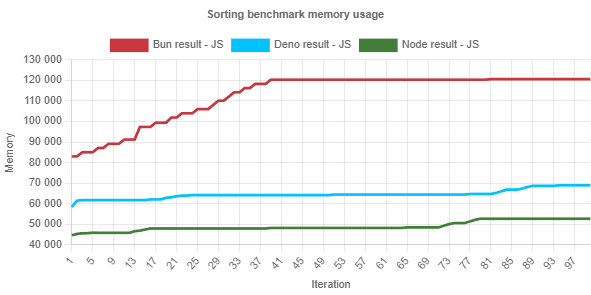
\includegraphics[width=0.8\textwidth]{Figures/sorting/quick/e2_memory_js.png}
  \caption{Wyniki eksperymentów dla algorytmu sortowania bąbelkowego dla 100 iteracji i 1000 elementów}
  \label{fig:quick_sorting_e2_memory_js}
\end{figure}

Na wykresie \ref{fig:quick_sorting_e2_ts} przedstawiono wyniki eksperymentu dla 100 iteracji oraz 1000 elementów dla algorytmów sortowania bąbelkowego napisanego w języku TypeScript. Na osi X przedstawia liczbę iteracji, na osi Y czas wykonania algorytmu w sekundach. 

\begin{figure}[H]
  \centering
  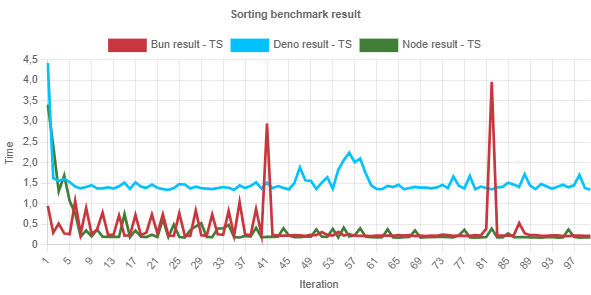
\includegraphics[width=0.8\textwidth]{Figures/sorting/quick/e2_ts.png}
  \caption{Wyniki eksperymentów dla algorytmu sortowania bąbelkowego dla 100 iteracji i 1000 elementów}
  \label{fig:quick_sorting_e2_ts}
\end{figure}

Na wykresie \ref{fig:quick_sorting_e2_memory_ts} przedstawiono wyniki eksperymentów dla algorytmu sortowania bąbelkowego dla 100 iteracji i 1000 elementów napisanego w języku TypeScript. Na osi X przedstawiono liczbę iteracji, natomiast na osi Y wykorzystanie pamięci w kilobytach. Jak widać, czas wykonania algorytmu rośnie wraz z ilością elementów.
\begin{figure}[H]
  \centering
  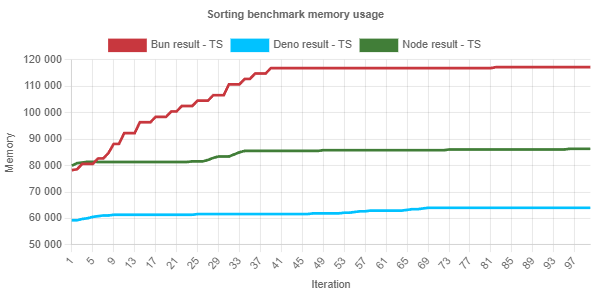
\includegraphics[width=0.8\textwidth]{Figures/sorting/quick/e2_memory_ts.png}
  \caption{Wyniki eksperymentów dla algorytmu sortowania bąbelkowego dla 100 iteracji i 1000 elementów}
  \label{fig:quick_sorting_e2_memory_ts}
\end{figure}

% 3
Na wykresie \ref{fig:quick_sorting_e3} przedstawiono wyniki eksperymentów dla algorytmu sortowania bąbelkowego dla 1000 iteracji oraz 1000 elementów napisanego w języku JavaScript. Na osi X przedstawiono liczbę iteracji, natomiast na osi Y wykorzystanie pamięci w kilobytach. Jak widać, czas wykonania algorytmu rośnie wraz z ilością elementów.
\begin{figure}[H]
  \centering
  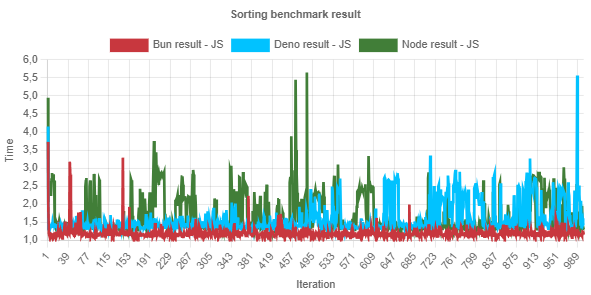
\includegraphics[width=0.8\textwidth]{Figures/sorting/quick/e3_js.png}
  \caption{Wyniki eksperymentów dla algorytmu sortowania bąbelkowego dla 1000 iteracji i 1000 elementów}
  \label{fig:quick_sorting_e3}
\end{figure}

Na wykresie \ref{fig:quick_sorting_e3_memory_js} przedstawiono wyniki eksperymentów dla algorytmu sortowania bąbelkowego dla 1000 iteracji oraz 1000 elementów napisanego w języku JavaScript. Na osi X przedstawiono liczbę iteracji, natomiast na osi Y wykorzystanie pamięci w kilobytach. Jak widać, czas wykonania algorytmu rośnie wraz z ilością elementów.
\begin{figure}[H]
  \centering
  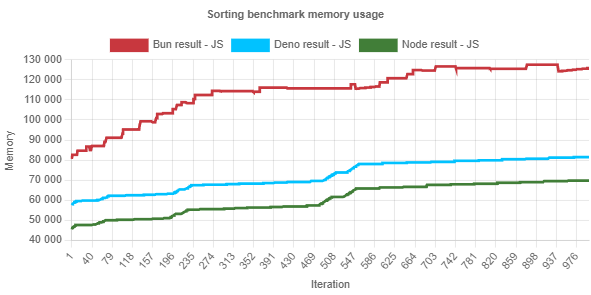
\includegraphics[width=0.8\textwidth]{Figures/sorting/quick/e3_memory_js.png}
  \caption{Wyniki eksperymentów dla algorytmu sortowania bąbelkowego dla 1000 iteracji i 1000 elementów}
  \label{fig:quick_sorting_e3_memory_js}
\end{figure}

Na wykresie \ref{fig:quick_sorting_e3_ts} przedstawiono wyniki eksperymentu dla 1000 iteracji oraz 1000 elementów dla algorytmów sortowania bąbelkowego, napisanego w języku TypeScript. Na osi X przedstawia liczbę iteracji, na osi Y czas wykonania algorytmu w sekundach. 

\begin{figure}[H]
  \centering
  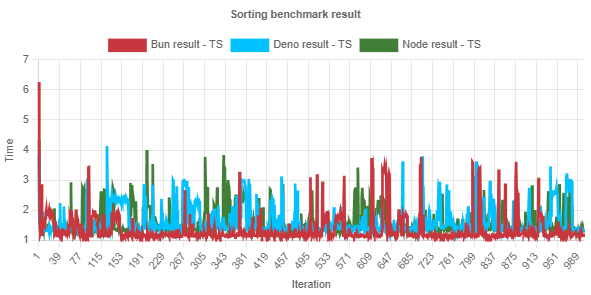
\includegraphics[width=0.8\textwidth]{Figures/sorting/quick/e3_ts.png}
  \caption{Wyniki eksperymentów dla algorytmu sortowania bąbelkowego dla 1000 iteracji i 1000 elementów}
  \label{fig:quick_sorting_e3_ts}
\end{figure}

Na wykresie \ref{fig:quick_sorting_e3_memory_ts} przedstawiono wyniki eksperymentów dla algorytmu sortowania bąbelkowego. Na osi X przedstawiono liczbę iteracji, natomiast na osi Y wykorzystanie pamięci w kilobytach. Jak widać, czas wykonania algorytmu rośnie wraz z ilością elementów.
\begin{figure}[H]
  \centering
  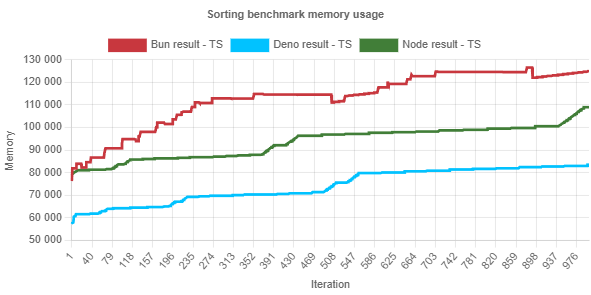
\includegraphics[width=0.8\textwidth]{Figures/sorting/quick/e3_memory_ts.png}
  \caption{Wyniki eksperymentów dla algorytmu sortowania bąbelkowego dla 1000 iteracji i 1000 elementów}
  \label{fig:quick_sorting_e3_memory_ts}
\end{figure}

%4
Na wykresie \ref{fig:quick_sorting_e4} przedstawiono wyniki eksperymentów dla algorytmu sortowania bąbelkowego. Na osi X przedstawiono liczbę iteracji, natomiast na osi Y wykorzystanie pamięci w kilobytach. Jak widać, czas wykonania algorytmu rośnie wraz z ilością elementów.
\begin{figure}[H]
  \centering
  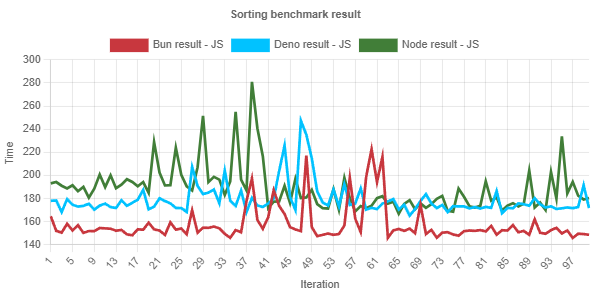
\includegraphics[width=0.8\textwidth]{Figures/sorting/quick/e4_js.png}
  \caption{Wyniki eksperymentów dla algorytmu sortowania bąbelkowego dla 10 iteracji i 10000 elementów}
  \label{fig:quick_sorting_e4}
\end{figure}

Na wykresie \ref{fig:quick_sorting_e4_memory_js} przedstawiono wyniki eksperymentów dla algorytmu sortowania bąbelkowego. Na osi X przedstawiono liczbę iteracji, natomiast na osi Y wykorzystanie pamięci w kilobytach. Jak widać, czas wykonania algorytmu rośnie wraz z ilością elementów.
\begin{figure}[H]
  \centering
  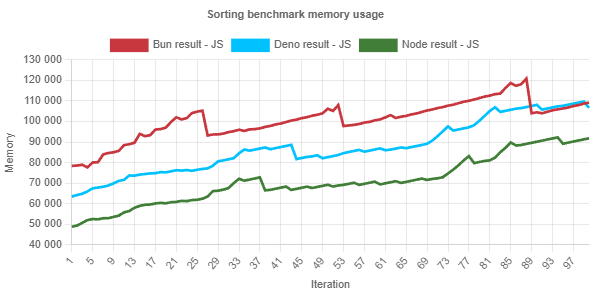
\includegraphics[width=0.8\textwidth]{Figures/sorting/quick/e4_memory_js.png}
  \caption{Wyniki eksperymentów dla algorytmu sortowania bąbelkowego dla 10 iteracji i 10000 elementów}
  \label{fig:quick_sorting_e4_memory_js}
\end{figure}

Na wykresie \ref{fig:quick_sorting_e4_ts} przedstawiono wyniki eksperymentu dla 100 iteracji oraz 1000 elementów dla algorytmów sortowania bąbelkowego. Na osi X przedstawia liczbę iteracji, na osi Y czas wykonania algorytmu w sekundach. 

\begin{figure}[H]
  \centering
  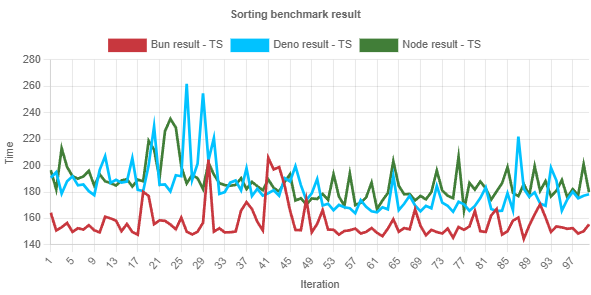
\includegraphics[width=0.8\textwidth]{Figures/sorting/quick/e4_ts.png}
  \caption{Wyniki eksperymentów dla algorytmu sortowania bąbelkowego dla 10 iteracji i 10000 elementów}
  \label{fig:quick_sorting_e4_ts}
\end{figure}

Na wykresie \ref{fig:quick_sorting_e4_memory_ts} przedstawiono wyniki eksperymentów dla algorytmu sortowania bąbelkowego. Na osi X przedstawiono liczbę iteracji, natomiast na osi Y wykorzystanie pamięci w kilobytach. Jak widać, czas wykonania algorytmu rośnie wraz z ilością elementów.
\begin{figure}[H]
  \centering
  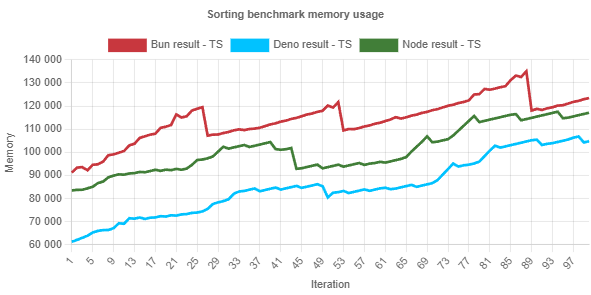
\includegraphics[width=0.8\textwidth]{Figures/sorting/quick/e4_memory_ts.png}
  \caption{Wyniki eksperymentów dla algorytmu sortowania bąbelkowego dla 10 iteracji i 10000 elementów}
  \label{fig:quick_sorting_e4_memory_ts}
\end{figure}

% 5
Na wykresie \ref{fig:quick_sorting_e5} przedstawiono wyniki eksperymentów dla algorytmu sortowania bąbelkowego. Na osi X przedstawiono liczbę iteracji, natomiast na osi Y wykorzystanie pamięci w kilobytach. Jak widać, czas wykonania algorytmu rośnie wraz z ilością elementów.
\begin{figure}[H]
  \centering
  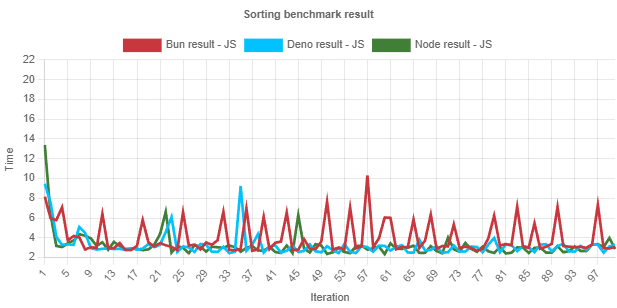
\includegraphics[width=0.8\textwidth]{Figures/sorting/quick/e5_js.png}
  \caption{Wyniki eksperymentów dla algorytmu sortowania bąbelkowego dla 100 iteracji i 10000 elementów}
  \label{fig:quick_sorting_e5}
\end{figure}

Na wykresie \ref{fig:quick_sorting_e5_memory_js} przedstawiono wyniki eksperymentów dla algorytmu sortowania bąbelkowego. Na osi X przedstawiono liczbę iteracji, natomiast na osi Y wykorzystanie pamięci w kilobytach. Jak widać, czas wykonania algorytmu rośnie wraz z ilością elementów.
\begin{figure}[H]
  \centering
  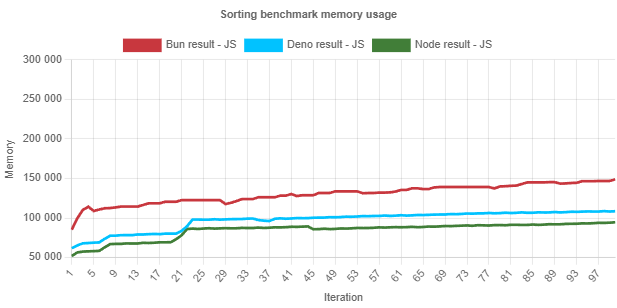
\includegraphics[width=0.8\textwidth]{Figures/sorting/quick/e5_memory_js.png}
  \caption{Wyniki eksperymentów dla algorytmu sortowania bąbelkowego dla 100 iteracji i 10000 elementów}
  \label{fig:quick_sorting_e5_memory_js}
\end{figure}

Na wykresie \ref{fig:quick_sorting_e5_ts} przedstawiono wyniki eksperymentu dla 100 iteracji oraz 1000 elementów dla algorytmów sortowania bąbelkowego. Na osi X przedstawia liczbę iteracji, na osi Y czas wykonania algorytmu w sekundach. 

\begin{figure}[H]
  \centering
  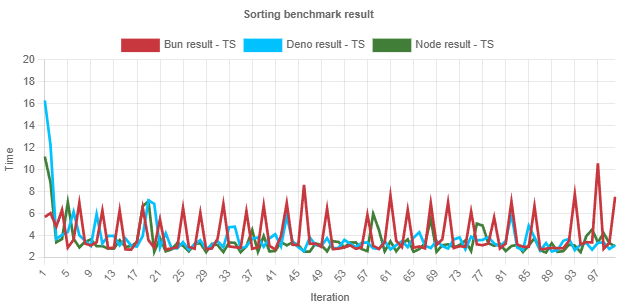
\includegraphics[width=0.8\textwidth]{Figures/sorting/quick/e5_ts.png}
  \caption{Wyniki eksperymentów dla algorytmu sortowania bąbelkowego dla 100 iteracji i 10000 elementów}
  \label{fig:quick_sorting_e5_ts}
\end{figure}

Na wykresie \ref{fig:quick_sorting_e5_memory_ts} przedstawiono wyniki eksperymentów dla algorytmu sortowania bąbelkowego. Na osi X przedstawiono liczbę iteracji, natomiast na osi Y wykorzystanie pamięci w kilobytach. Jak widać, czas wykonania algorytmu rośnie wraz z ilością elementów.
\begin{figure}[H]
  \centering
  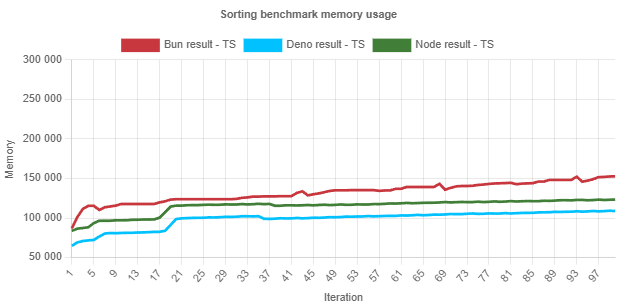
\includegraphics[width=0.8\textwidth]{Figures/sorting/quick/e5_memory_ts.png}
  \caption{Wyniki eksperymentów dla algorytmu sortowania bąbelkowego dla 100 iteracji i 10000 elementów}
  \label{fig:quick_sorting_e5_memory_ts}
\end{figure}

% 6
Na wykresie \ref{fig:quick_sorting_e6} przedstawiono wyniki eksperymentów dla algorytmu sortowania bąbelkowego. Na osi X przedstawiono liczbę iteracji, natomiast na osi Y wykorzystanie pamięci w kilobytach. Jak widać, czas wykonania algorytmu rośnie wraz z ilością elementów.
\begin{figure}[H]
  \centering
  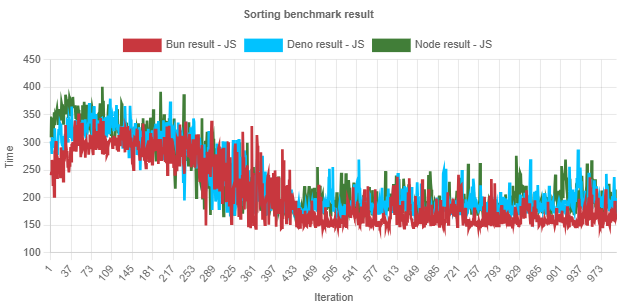
\includegraphics[width=0.8\textwidth]{Figures/sorting/quick/e6_js.png}
  \caption{Wyniki eksperymentów dla algorytmu sortowania bąbelkowego dla 1000 iteracji i 10000 elementów}
  \label{fig:quick_sorting_e6}
\end{figure}

Na wykresie \ref{fig:quick_sorting_e6_memory_js} przedstawiono wyniki eksperymentów dla algorytmu sortowania bąbelkowego. Na osi X przedstawiono liczbę iteracji, natomiast na osi Y wykorzystanie pamięci w kilobytach. Jak widać, czas wykonania algorytmu rośnie wraz z ilością elementów.
\begin{figure}[H]
  \centering
  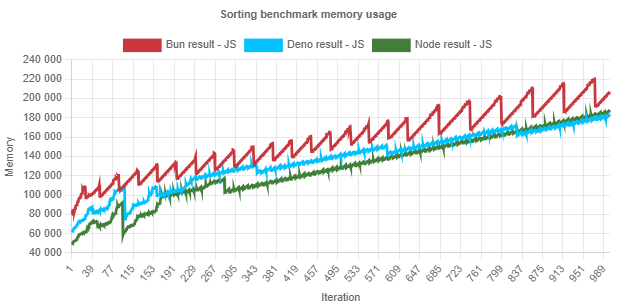
\includegraphics[width=0.8\textwidth]{Figures/sorting/quick/e6_memory_js.png}
  \caption{Wyniki eksperymentów dla algorytmu sortowania bąbelkowego dla 1000 iteracji i 10000 elementów}
  \label{fig:quick_sorting_e6_memory_js}
\end{figure}

Na wykresie \ref{fig:quick_sorting_e6_ts} przedstawiono wyniki eksperymentu dla 100 iteracji oraz 1000 elementów dla algorytmów sortowania bąbelkowego. Na osi X przedstawia liczbę iteracji, na osi Y czas wykonania algorytmu w sekundach. 

\begin{figure}[H]
  \centering
  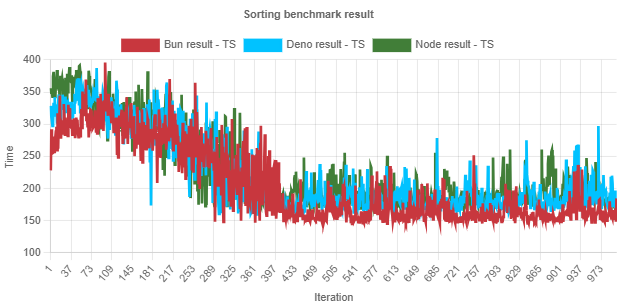
\includegraphics[width=0.8\textwidth]{Figures/sorting/quick/e6_ts.png}
  \caption{Wyniki eksperymentów dla algorytmu sortowania bąbelkowego dla 1000 iteracji i 10000 elementów}
  \label{fig:quick_sorting_e6_ts}
\end{figure}

Na wykresie \ref{fig:quick_sorting_e6_memory_ts} przedstawiono wyniki eksperymentów dla algorytmu sortowania bąbelkowego. Na osi X przedstawiono liczbę iteracji, natomiast na osi Y wykorzystanie pamięci w kilobytach. Jak widać, czas wykonania algorytmu rośnie wraz z ilością elementów.
\begin{figure}[H]
  \centering
  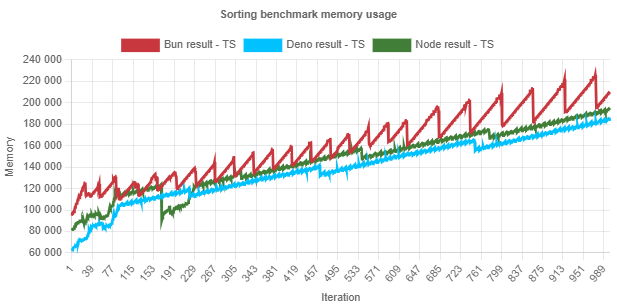
\includegraphics[width=0.8\textwidth]{Figures/sorting/quick/e6_memory_ts.png}
  \caption{Wyniki eksperymentów dla algorytmu sortowania bąbelkowego dla 1000 iteracji i 10000 elementów}
  \label{fig:bubble_sorting_e6_memory_ts}
\end{figure}

\subsubsection{Wyniki - sortowanie pozycyjne}

\subsection{Algorytmy kodowania}

\subsubsection{Wyniki}

\subsection{Testy wydajnościowe operacji zapisu i odczytu plików}

\subsubsection{Wyniki}

\subsection{Testy wydajnościowe serwera HTTP}

\subsubsection{Wyniki}

\subsection{Testy wydajnościowe zapisu i odczytu danych z bazy danych}

\subsubsection{Wyniki}